\documentclass[11pt]{beamer}
\usepackage{graphicx,hyperref}
\usepackage{subfigure}
\usepackage[english]{babel}
\usepackage{times}
\usepackage[T1]{fontenc}
\usepackage{diagbox}
\usepackage[authordate]{biblatex-chicago}
\usepackage{setspace}
\usepackage{chngcntr}
\usepackage[table]{xcolor}
\usepackage{appendixnumberbeamer}
\usepackage{tikz}
\usepackage{csquotes}
\usepackage{longtable}
\usepackage{booktabs}

\newcommand{\E}{\mathbb{E}}
\newcommand{\Prob}{\mathbb{P}}
\newcommand{\ind}[1]{\mathbf{1}\!\left\{#1\right\}}
\newcommand{\Ehat}{\widehat{\E}}
\newcommand{\Phat}{\widehat{\Prob}}
\newcommand{\ATT}{\mathrm{ATT}}
\newcommand{\CATT}{\mathrm{CATT}}
\newcommand{\Logit}{\Lambda}
\newcommand{\DY}[2]{\Delta Y_i^{(#1,#2)}}

\usetikzlibrary{arrows,positioning} 
\tikzset{
    %Define standard arrow tip
    >=stealth',
    %Define style for boxes
    punkt/.style={
           rectangle,
           rounded corners,
           draw=black, very thick,
           text width=6.5em,
           minimum height=2em,
           text centered},
    % Define arrow style
    pil/.style={
           ->,
           thick,
           shorten <=2pt,
           shorten >=2pt,}
}
\usepackage{hyperref}
\addbibresource{bib/PoliceResidency.bib}


\usetheme{Madrid}
\definecolor{EmoryBlue}{RGB}{1,33,105}
\usecolortheme[named=EmoryBlue]{structure}



    \title[Estimator Selection]{Estimator Selection Diagnostics in Staggered Differences-in-Differences}
    \author[Eric Dobbie]{Eric Dobbie}
    \institute[Emory]{Emory University\\Department of Political Science} 
    \date{\today}  
    \logo{
\includegraphics[width=1.19cm,height=0.4cm]{slidefigures/School.png}}

\begin{document}
%%%%%%%%%%%%%%%%%%%%%%%%%%%%%%%%%%%%%%%%%%%%%%%%%%%%%%%%%%%%%%%%%%%%%%%%%%%%%%%%%%%%%%
\begin{frame}\titlepage
\end{frame}

\section{Background}

\begin{frame}{Staggered Treatment DiD}
    \begin{itemize}
        \item Common applied DiD settings are complicated, with treatments being applied at different time periods for different geographic units.
        \item These setting are especially common in policy evaluation settings, where policy is not adopted uniformly across different jurisdictions.
        \item Typical applied work used TWFE estimators in these applications
    \end{itemize}
\end{frame}

\section{Staggered Treatments Lead to Bad Comparisons}

\begin{frame}{Goodman-Bacon Bias}
    \begin{itemize}
        \item However, TWFE has a problem. \textcite{goodman2021difference} showed that using TWFE leads to unintuitive comparisons, where the treatment group in a previous period serves as the control group for units treated in the current period.
        \item These comparisons bias the estimate of the ATT when using TWFE models
    \end{itemize}

    The bias term is given by 
    \begin{equation}\label{eq:biastwfe}
        \text{Bias} = \sum_{k \not = U} \sum_{\mathcal{L} > k} \sigma_{k \mathcal{L}} (1 - \mu_{k\mathcal{L}})[ATT_k(POST(\mathcal{L})) - ATT_k(MID(k,\mathcal{L}))]
    \end{equation}
    Which is the change in treatment effect across periods.
\end{frame}

\section{Goodman-Bacon Decomposition}

\begin{frame}{Goodman-Bacon Decomposition}
    \textcite{goodman2021difference} decomposes the TWFE model into all possible 2x2 DiD comparisons.

    \begin{figure}
        \centering
        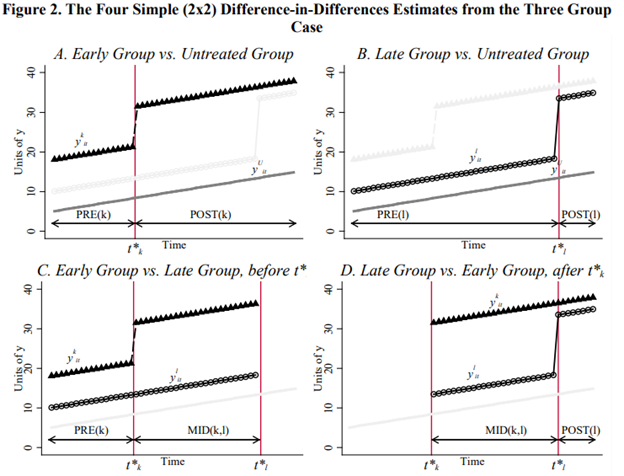
\includegraphics[width=0.7\linewidth]{slidefigures/comparisons.png}
        \label{fig:GB_Decomp}
    \end{figure}
\end{frame}

\begin{frame}{Goodman-Bacon Decomposition}
    There are two (related) problems that arise from this:

    \begin{enumerate}
        \item Some of these comparisons (namely Panel D) are unintuitive, strange comparisons
        \item When we include these strange comparisons, the weights on some of these 2x2 DiD cells can be negative in the aggregation process, leading to biased estimates.
    \end{enumerate}

     Because of these problems, TWFE estimators are generally not advisable in staggered treatment settings
\end{frame}

\section{Reweighting Estimators}

\begin{frame}{The Solution: Restrict Focus to Clean Comparisons}
    There is a class of modern estimators that works by restricting the analysis to clean comparisons of treated groups with not-yet-treated or never-treated control groups.

    \vspace{2.5mm}

    For this paper I will focus on the most widely adopted set of these estimators (\cite{callaway2021difference, sun2021estimating})
\end{frame}


\begin{frame}{How do reweighting estimators work?}
    Imagine a setting with $n$ treatment cohorts and $m$ time periods.
    
    \vspace{2.5mm}

    \begin{table}[]
\centering
\begin{tabular}{c|ccccc}
      \diagbox{g}{j}   & 1              & 2              & ...      & m-1              & m              \\ \hline
1        & $\tau_{1,1}$   & $\tau_{1,2}$   & ...      & $\tau_{1,m-1}$   & $\tau_{1,m}$   \\
2        & 0   & $\tau_{2,2}$   & ...      & $\tau_{2,m-1}$   & $\tau_{2,m}$   \\
$\vdots$ & $\vdots$       & $\vdots$       & $\vdots$ & $\vdots$         & $\vdots$       \\
n-1      & 0 & 0 & ...      & $\tau_{n-1,m-1}$ & $\tau_{n-1,m}$ \\
n        & 0  & 0   & ...      & $\tau_{n,m-1}$   & $\tau_{n,m}$  
\end{tabular}
\end{table}

    With treatment in period $k_g$, let $g \in [1,n]$ index treatment cohorts and $j \in [1,m]$ index time period, where $j \in [1,k_g)$ represent pre-treatment periods for each cohort and $j \in [k_g,m]$ represent treated periods. Each $\ tau_{g,j}$ represents the cohort by period ATT.

\end{frame}

\begin{frame}{What is each $\tau$?}
    $\tau_{g,j}$ is the average treatment effect among the units of cohort $g$ in time $j$.
\end{frame}

\begin{frame}{Aggregating to the ATT}    
    \textcite{callaway2021difference} propose that researchers should use these as a target estimand and directly report these $\ tau_{g,j}$ values. 

    \vspace{2.5mm}
    
    However, in settings where $g$ and/or $j$ are large, the number of $\ tau_{g,j}$ values will be too large to take away substantive conclusions. 
    
\vspace{2.5mm}
    
    Therefore, many applied researchers look to aggregate these cohort by period effects into a more familiar aggregate ATT.
\end{frame}


\begin{frame}{Reasonable Aggregation Schemes}
    In order to aggregate these $\ tau_{g,j}$ estimates, one can imagine several possible approaches:

    \begin{itemize}
        \item Aggregating over cohorts to generate event study or calendar estimates with period specific effects
        \item Aggregating over periods to generate cohort specific effects
        \item Aggregating over both periods and cohorts to generate a single ATT
    \end{itemize}
\end{frame}


\begin{frame}{Event Study Aggregation}
    For event study aggregation, the target is to reduce from $\ tau_{g,j}$ to period specific effects, $\theta_{es}(e)$, where $e$ represents the number of periods since treatment for each cohort $g$. Formally, $e = j - k_g$. The event study estimate is given by:
    \begin{equation}
        \theta_{es}(e) = \sum_i w_{i,e} \ tau_{g,e}
    \end{equation}

    Note that $e$ is cohort specific, such that $e = 1$ can be in different time periods $j$ for each cohort. 
\end{frame}

\begin{frame}{Event Study Aggregation}
    Consider an example with 5 time periods and 4 treatment cohorts, treated in periods 2 to 5 sequentially, such that cohort 1 is treated in period 2, cohort 2 is treated in period 3, and so on.
    \begin{table}[]
\centering
\begin{tabular}{c|ccccc}
      \diagbox{i}{j}   & 1              & 2              & 5      & 4             & 5              \\ \hline
1        & $\tau_{1,1}$   & $\tau_{1,2}$   & $\tau_{1,3}$    & $\tau_{1,4}$   & $\tau_{1,5}$   \\
2        & $\tau_{2,1}$   & $\tau_{2,2}$   & $\tau_{2,3}$      & $\tau_{2,4}$   & $\tau_{2,5}$   \\
3      & $\tau_{3,1}$ & $\tau_{3,2}$ &  $\tau_{3,3}$     & $\tau_{3,4}$ & $\tau_{3,5}$ \\
4        & $\tau_{4,1}$   & $\tau_{4,2}$   & $\tau_{4,3}$     & $\tau_{4,4}$   & $\tau_{4,5}$  
\end{tabular}
\end{table}
\end{frame}

\begin{frame}{Event Study Aggregation}
    To estimate $\theta_{es}(1)$, the blue cells are added together using a weighted average, $\theta_{es}(2)$ is a weighted average of green cells, $\theta_{es}(3)$ is a weighted average of the purple cells, and $\theta_{es}(4) = \tau_{1,5}$, the orange cell, by construction:

    \begin{table}[]
\centering
\begin{tabular}{c|ccccc}
      \diagbox{g}{j}   & 1              & 2              & 3      & 4             & 5              \\ \hline
1        & 0   &\cellcolor{blue!30} $\tau_{1,2}$   & \cellcolor{green!30}$\tau_{1,3}$    & \cellcolor{purple!30}$\tau_{1,4}$   &\cellcolor{orange!30} $\tau_{1,5}$   \\
2        & 0   & 0  & \cellcolor{blue!30}$\tau_{2,3}$      & \cellcolor{green!30}$\tau_{2,4}$   & \cellcolor{purple!30}$\tau_{2,5}$   \\
3      & 0 & 0 &  0     & \cellcolor{blue!30}$\tau_{3,4}$ & \cellcolor{green!30}$\tau_{3,5}$ \\
4        & 0  & 0   & 0     & 0   & \cellcolor{blue!30}$\tau_{4,5}$  
\end{tabular}
\end{table}
\end{frame}

\begin{frame}{Event Study Aggregation}
    The weights, $w_{i,e}$, depend on the estimator. \textcite{sun2021estimating} weigh by cohort-period shares such that, in the example:
    \begin{equation}
        \theta_{es}(e) = \frac{n_{i=1, e}}{n_{e}} \tau_{1,e} + \frac{n_{i=2, e}}{n_{e}} \tau_{2,e}+\frac{n_{i=3, e}}{n_{e}} \tau_{3,e}+\frac{n_{i=4, e}}{n_{e}} \tau_{4,e}
    \end{equation}

    Where $\frac{n_{i,e}}{n_e}$ is the share of that event period sample size from that treatment cohort. For $e = 2$, for example:

    \begin{align*}
                \theta_{es}(2) &= \frac{n_{i=1, 2}}{n_{2}} \tau_{1,2} + \frac{n_{i=2, 2}}{n_{2}} \tau_{2,2}+\frac{n_{i=3, e}}{n_{2}} \tau_{3,e}+\frac{0}{n_{2}} \tau_{4,2} \\
                & = \frac{n_{i=1, 2}}{n_{2}} \tau_{1,2} + \frac{n_{i=2, 2}}{n_{2}} \tau_{2,2}+\frac{n_{i=3, e}}{n_{2}} \tau_{3,e}
    \end{align*}
\end{frame}

\begin{frame}{Calendar Effects}
    Another approach uses a calendar specific aggregation. Instead of normalizing to event time, one might be interested in the treatment effect at different points in time, so we aggregate over treatment cohorts within period $j$, for each cohort $g$ such that $j > k_g$.
    \begin{equation}
        \theta_c(j) = \sum_{g;j > k_g} w_{g,j} \ tau_{g,j}
    \end{equation}
\end{frame}

\begin{frame}{Calendar Effects}
    Carrying forward the previous example,  $\theta_{c}(1) = \tau_{1,2}$, the blue cell, $\theta_{c}(2)$ is a weighted average of green cells, $\theta_{c}(3)$ is a weighted average of the purple cells, and $\theta_{c}(4)$ is a weighted average of the orange the orange cells.

    \input{tables/calendar/ex_cal}
\end{frame}

\begin{frame}{Cohort Specific Effects}
    One could similarly imagine being interested in estimating the effects of a policy on each treatment cohort. For this, one would want to aggregate across time periods. 

    \begin{equation}
        \alpha_i = \sum_{j > k_i} w_{i,j} \ tau_{g,j}
    \end{equation}
\end{frame}

\begin{frame}{Cohort Specific Effects}
    Returning to the example, to find cohort effects we aggregate over time within cohorts, so $\alpha_1$ is a weighted average of the blue cells, $\alpha_2$ is a weighted average of the green cells, $\alpha_3$ is a weighted average of the purple cells, and $\alpha_4 = \tau_{4,5}$, the orange cell.
    \begin{table}[]
\centering
\begin{tabular}{c|ccccc}
      \diagbox{i}{j}   & 1              & 2              & 3      & 4             & 5              \\ \hline
1        & $\tau_{1,1}$   &\cellcolor{blue!30} $\tau_{1,2}$   & \cellcolor{blue!30}$\tau_{1,3}$    & \cellcolor{blue!30}$\tau_{1,4}$   &\cellcolor{blue!30} $\tau_{1,5}$   \\
2        & $\tau_{2,1}$   & $\tau_{2,2}$   & \cellcolor{green!30}$\tau_{2,3}$      & \cellcolor{green!30}$\tau_{2,4}$   & \cellcolor{green!30}$\tau_{2,5}$   \\
3      & $\tau_{3,1}$ & $\tau_{3,2}$ &  $\tau_{3,3}$     & \cellcolor{purple!30}$\tau_{3,4}$ & \cellcolor{purple!30}$\tau_{3,5}$ \\
4        & $\tau_{4,1}$   & $\tau_{4,2}$   & $\tau_{4,3}$     & $\tau_{4,4}$   & \cellcolor{orange!30}$\tau_{4,5}$  
\end{tabular}
\end{table}
\end{frame}

\begin{frame}{Single ATT Aggregation}
    The ATT for each of these reweighting estimators follows this general form:

    \begin{equation}\label{eq:delta}
        \delta = \sum_{i,j>k} w_{ij} * \ tau_{gj}
    \end{equation}

    Where $w_{i,j} > 0$ and $\sum_{i,j} w_{i,j} = 1$
\end{frame}

\begin{frame}{Single ATT Aggregation}
    To obtain a single ATT, all treated cells are combined using a weighted average to estimate $\delta$

    \input{tables/att/att}
\end{frame}

\section{Estimation}

\begin{frame}{Estimation of $\hat{\tau}_{g,t}$}
    Each of these three estimators uses a distinct approach to estimation of $\hat{\tau}_{g,t}$.

    \vspace{2mm}

    First, \cite{callaway2021difference} uses the following procedure:
    \begin{enumerate}
        \item Restrict the data to a subexperiment where we keep only units in
              cohort $g$ and the selected control group (never-treated or
              not-yet-treated), and periods $s = \{g-1,\, t\}$.
        \item Estimate propensity scores on that subsample $\mathcal{S}_{g,t}$:
    \end{enumerate}

    \vspace{-2mm}
    {\small
    \begin{align*}
      \hat\beta_{g,t}
        &= \arg\max_{\beta} \sum_{k \in \mathcal{S}_{g,t}}
           \Big[\, G_{g,k}\log \Lambda(X_k'\beta) \\[-0.5mm]
        &\hspace{26mm}
           + (1 - G_{g,k}) \log\big(1 - \Lambda(X_k'\beta)\big) \Big] \\[1mm]
      \hat\pi_{g,t}(X_k)
        &= \Lambda(X_k'\hat\beta_{g,t})
           \;\approx\; \Pr\big(G_{g,k} = 1 \mid X_k,\ G_{g,k} + C_k = 1\big)
    \end{align*}
    }
\end{frame}

\begin{frame}{Estimation of $\hat{\tau}_{g,t}$}
    \begin{enumerate}
        \item[3.] Fit an outcome model on control units only:
    \end{enumerate}

    \vspace{-2mm}
    {\small
    \begin{align*}
      \hat\gamma_{g,t}
        &= \arg\min_{\gamma} \sum_{k \in \mathcal{S}_{g,t}}
           C_k \, \frac{\hat\pi_{g,t}(X_k)}{1 - \hat\pi_{g,t}(X_k)}
           \Big( \Delta Y_k^{(g,t)} - X_k'\gamma \Big)^{2} \\[1mm]
      \hat\mu^{C}_{g,t}(X_k) &= X_k'\hat\gamma_{g,t}
    \end{align*}
    }

    \vspace{1mm}
    \begin{enumerate}
        \item[4.] Estimate the sub-experiment DiD with a doubly robust estimator.
              Writing $\hat o_k = \hat\pi_{g,t}(X_k) / \big(1 - \hat\pi_{g,t}(X_k)\big)$
              for the odds weight,
    \end{enumerate}

    \vspace{-2mm}
    {\small
    \begin{equation*}
      \widehat{\text{ATT}}^{\,dr}(g,t)
      = \frac{1}{n} \sum_{k \in \mathcal{S}_{g,t}}
        \left( \frac{G_{g,k}}{\widehat{\mathbb{E}}[G_g]}
             - \frac{\hat o_k \, C_k}{\widehat{\mathbb{E}}[\hat o \, C]} \right)
        \Big( \Delta Y_k^{(g,t)} - \hat\mu^{C}_{g,t}(X_k) \Big)
    \end{equation*}
    }
\end{frame}

\begin{frame}{Estimation of $\hat{\tau}$}

\cite{sun2021estimating} have a distinct approach, estimating one interactive model on the full sample:

\begin{align*}
  Y_{it}
  \;&=\;
  \alpha_i + \lambda_t
  + \sum_{g \notin C} \; \sum_{\ell \neq -1}
    \delta_{g,\ell} \Big( \ind{G_i = g} \cdot \ind{t - g = \ell} \Big)
  + \varepsilon_{it}, \\
  &\qquad
  \widehat{\CATT}_{g,\ell} \;=\; \hat\delta_{g,\ell}.
\end{align*}

    
\end{frame}

\section{Stacked Regression}

\begin{frame}{Stacked Regression: Process}

In order to run a stacked regression (\cite{cengiz2019effect}):

\begin{enumerate}
    \item Select a window around treatment for for the selection of clean controls, with equal number of periods before and after treatment.
    \item Identify clean controls based on selected control group (not-yet-treated or never-treated)
    \item Generate the ``stack'' with all units treated in time $t$ with all clean controls in the window selected.
\end{enumerate}

Once each stack has been formed, they are row binded together to form a full stacked dataset.
    
\end{frame}

\begin{frame}{Stacked Regression: Estimation}
    The standard stacked regression setup then uses a two-way fixed effect estimator:

    \begin{equation}
        Y_{i,t} = \alpha_{i,s} + \gamma_{t,s} + \delta D_{i,t,s} + \epsilon
    \end{equation}

    where: 
    
    \begin{itemize}
        \item $\alpha_{i,s}$ is a unit by stack fixed effect
        \item $\gamma_{t,s}$ is a year by stack fixed effect
        \item $\delta$ is the ATT estimate.
    \end{itemize}
\end{frame}

\begin{frame}{Reconstructing P\&P}

I used the standard stacked regression approach to reconstruct the stacked dataset. Without access to the code they used to build the stacked dataset for \cite{payson2023resreq}, which is not included in their replication files, I need to test some of the assumptions.
    
\end{frame}

\begin{frame}{Variation in Dataset Size by Assumptions}
    \input{tables/stacked_dimensionality_a}
\end{frame}

\begin{frame}{P\&P Stacked Regression}
    Adding them to the table of sample size by assumptions:

    \begin{table}[t]
\centering
\label{tab:stacked-dim-b}
\begin{tabular}{llr}
\toprule
Control group & Window (yrs before / after) & Rows \\
\midrule
Never-treated  & 4 / 4 & 40,140 \\
 & 5 / 5 & 40,898 \\
 & 6 / 6 & 48,334 \\
 & 7 / 7 & 44,640 \\
 P\&P & No window & 171,444 \\
\midrule
Not-yet-treated  & 4 / 4 & 40,644 \\
 & 5 / 5 & 41,173 \\
 & 6 / 6 & 48,581 \\
 & 7 / 7 & 44,895 \\
\bottomrule
\end{tabular}
\caption{Dimensionality of the stacked dataset under alternative window and clean-control-group assumptions.}
\end{table}

\end{frame}

\begin{frame}{P\&P Stacked Regression}

What assumptions did Payson and Parinandi make?
\begin{itemize}
    \item They used never-treated controls
    \item They use all clean control units rather than those that are clean within a window.
\end{itemize}

The second assumption here is nonstandard.
    
\end{frame}

\begin{frame}{The standard assumptions break the result}

Using the standard window based approach does lead to the results losing signigicance.

\begin{figure}
    \centering
    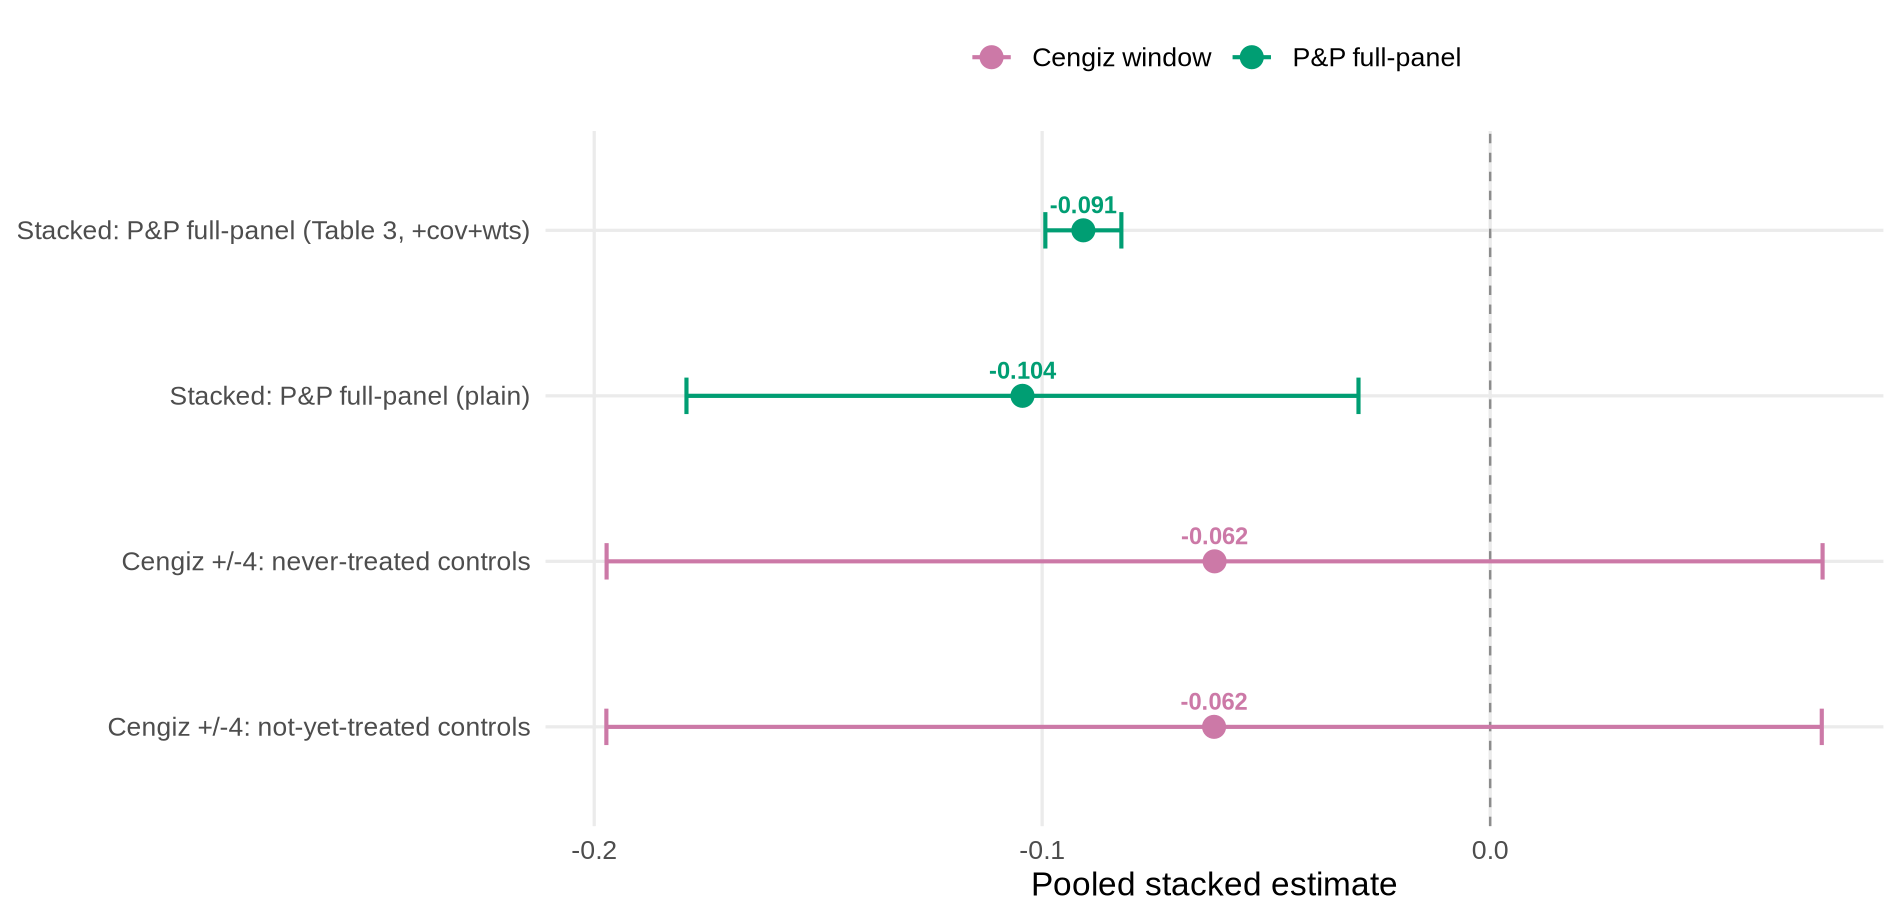
\includegraphics[width=0.75\linewidth]{figures/cengiz_control_groups.png}
    \label{fig:cengiz}
\end{figure}
    
\end{frame}

\begin{frame}{Does the window really matter?}

Not particularly. The coefficient is always negative but converges towards the P\&P result as the window length increases, but never regains significance due to the loss in sample size from the missing data boundary at 2000.

\begin{figure}
    \centering
    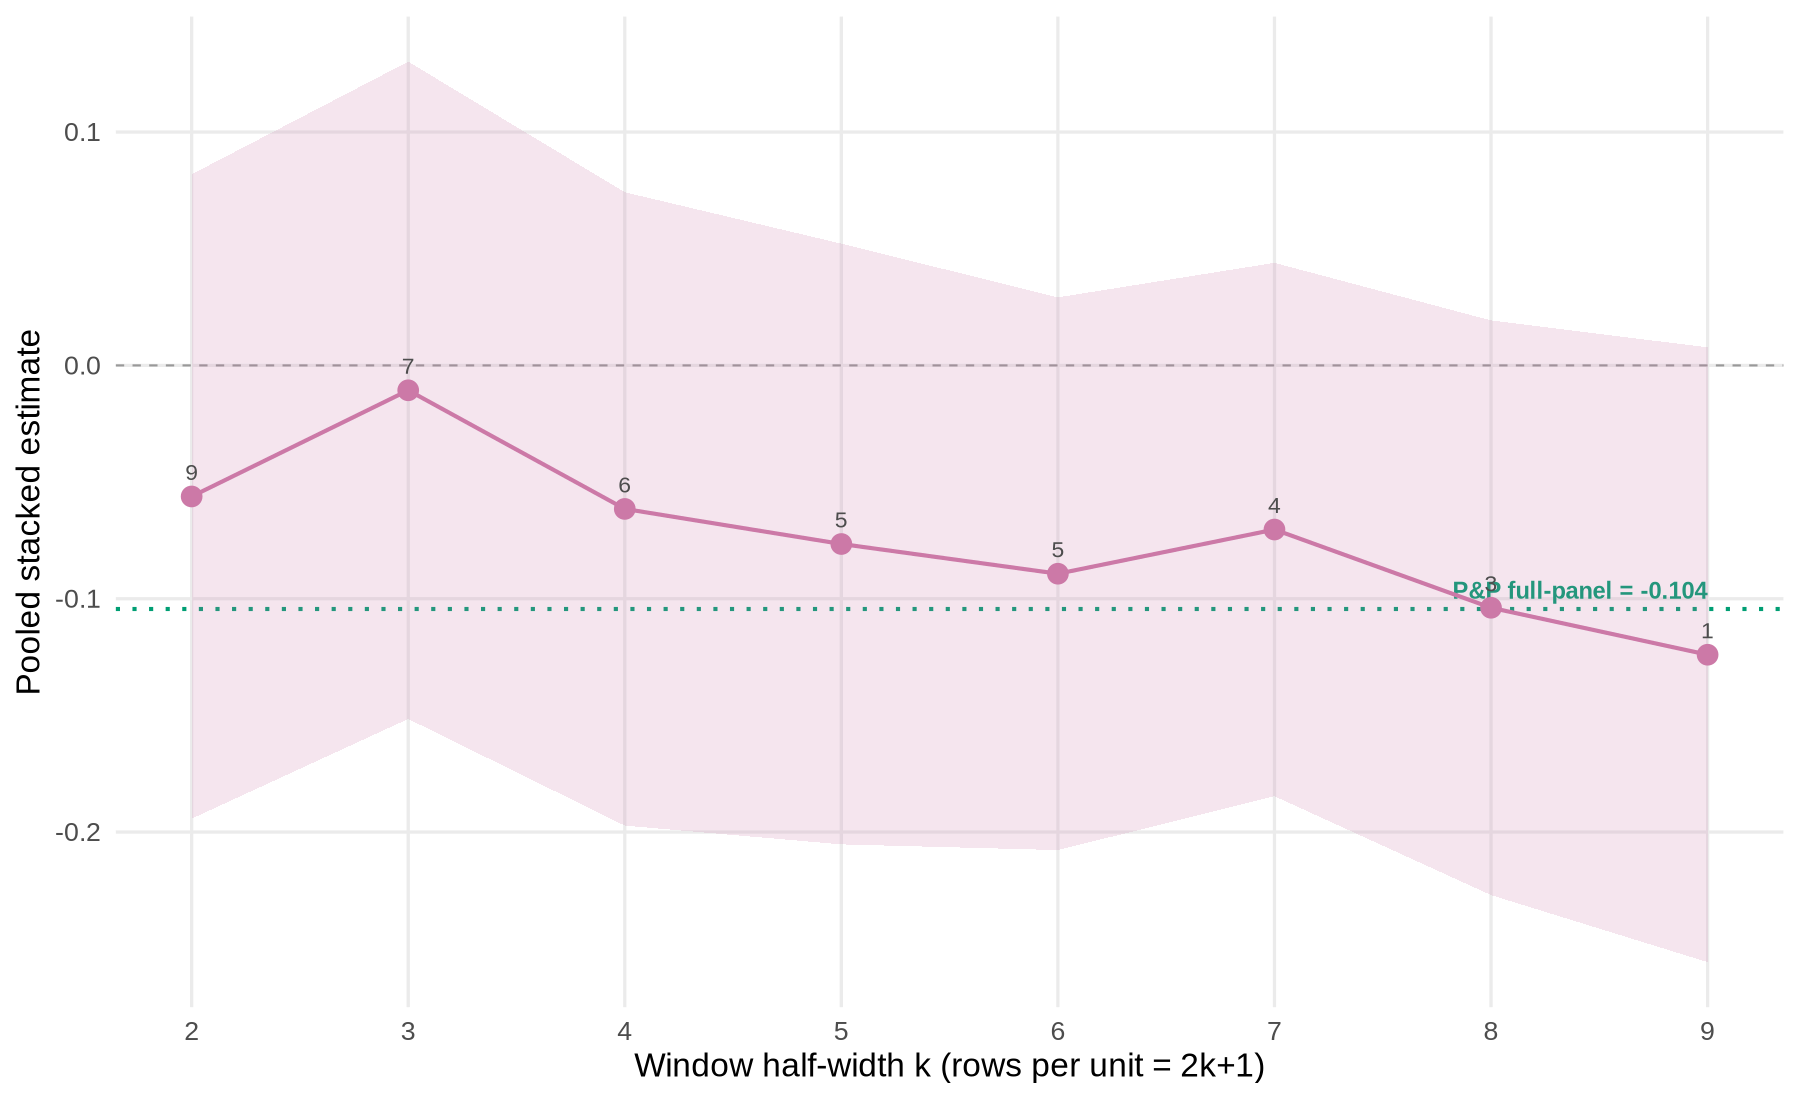
\includegraphics[width=0.75\linewidth]{figures/cengiz_window_sensitivity.png}
    \label{fig:window}
\end{figure}
    
\end{frame}

\begin{frame}{An estimation problem}
    In the process of replicating their approach, I found a (minor) coding error that is worth mentioning. They estimate the following:

    \begin{equation}
         Y_{i,t} = \alpha_{i} + \gamma_{t,s} + \delta D_{i,t,s} + \epsilon
    \end{equation}

    Where $\alpha_i$ is a unit fixed effect rather than a unit by cohort fixed effect. This means that the unit means for the fixed effect are residualized across the full panel, which masks the stack level effect heterogeneity.
\end{frame}

\begin{frame}{Correcting the Estimation Problem}
    \begin{figure}
        \centering
        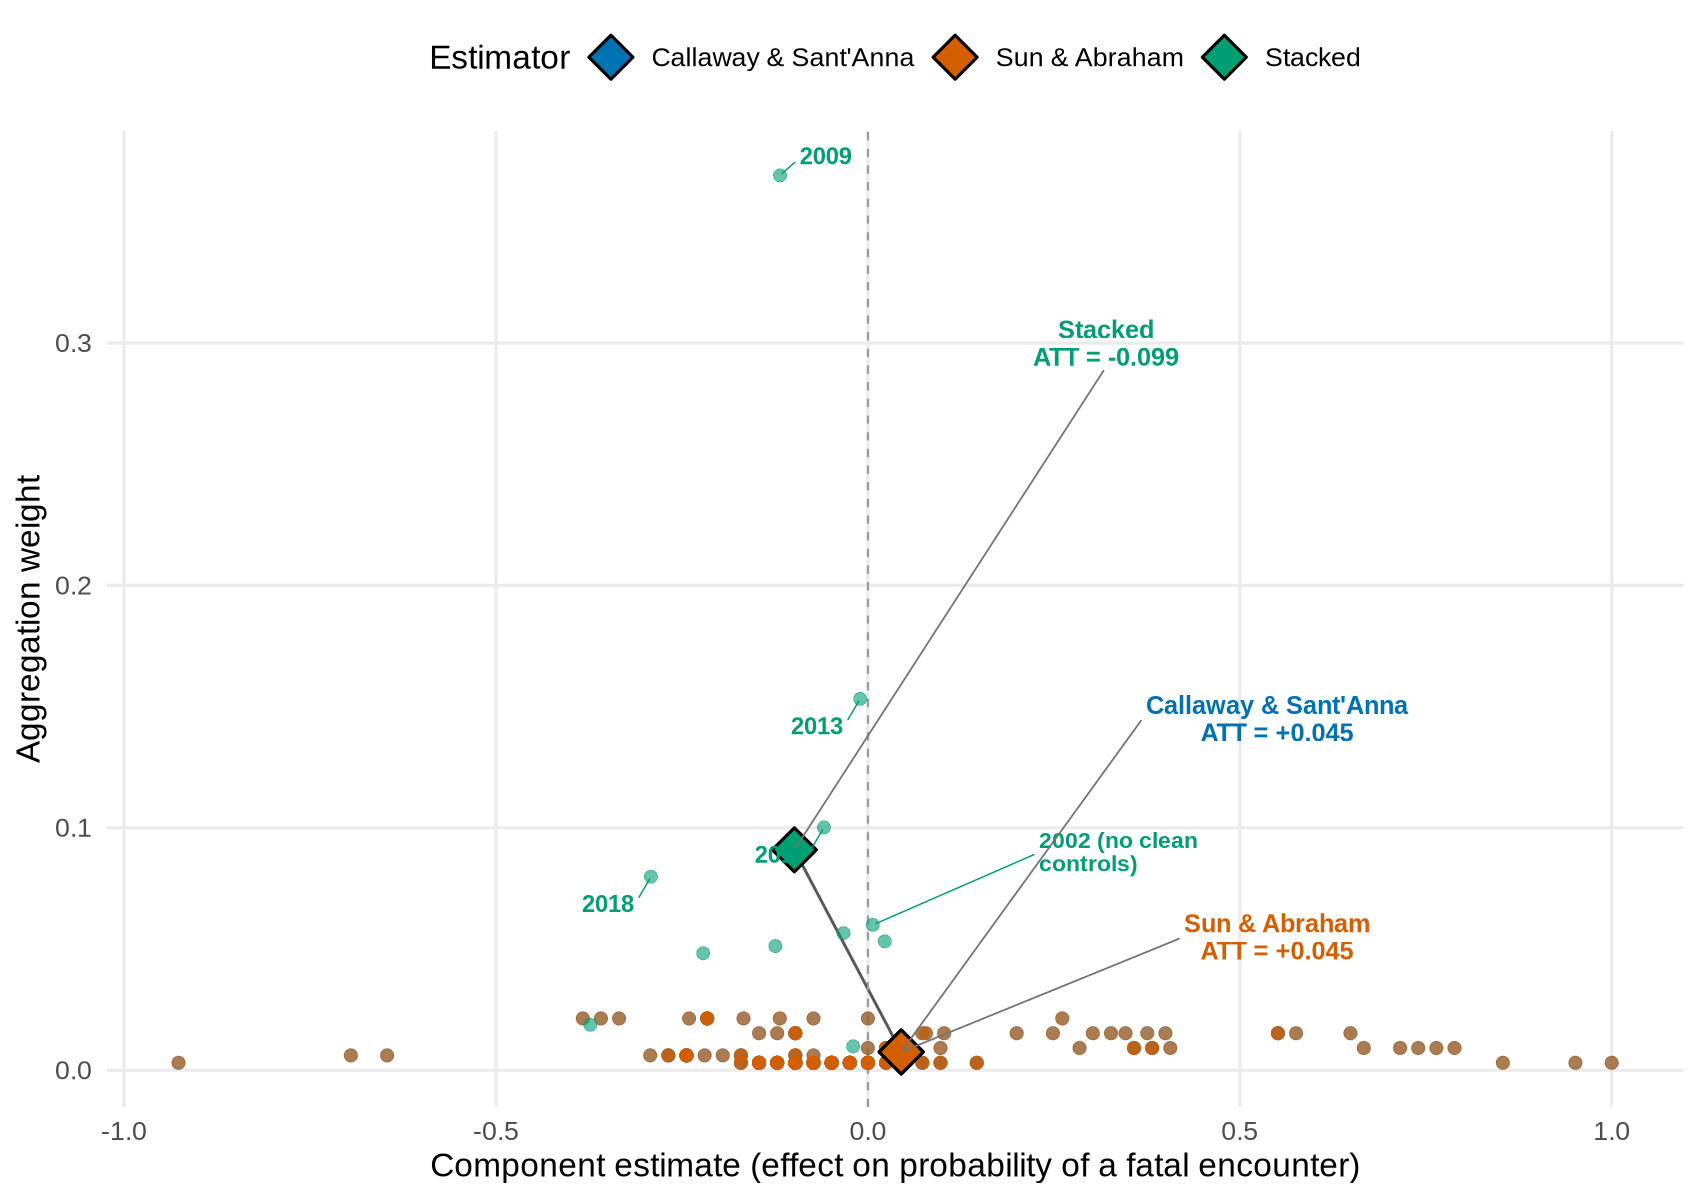
\includegraphics[width=0.6\linewidth]{figures/weight_vs_beta_decomposition.png}
        \label{fig:weights_points}
    \end{figure}
\end{frame}

\begin{frame}{Breaking out Estimates by Estimator}
    \begin{figure}
        \centering
        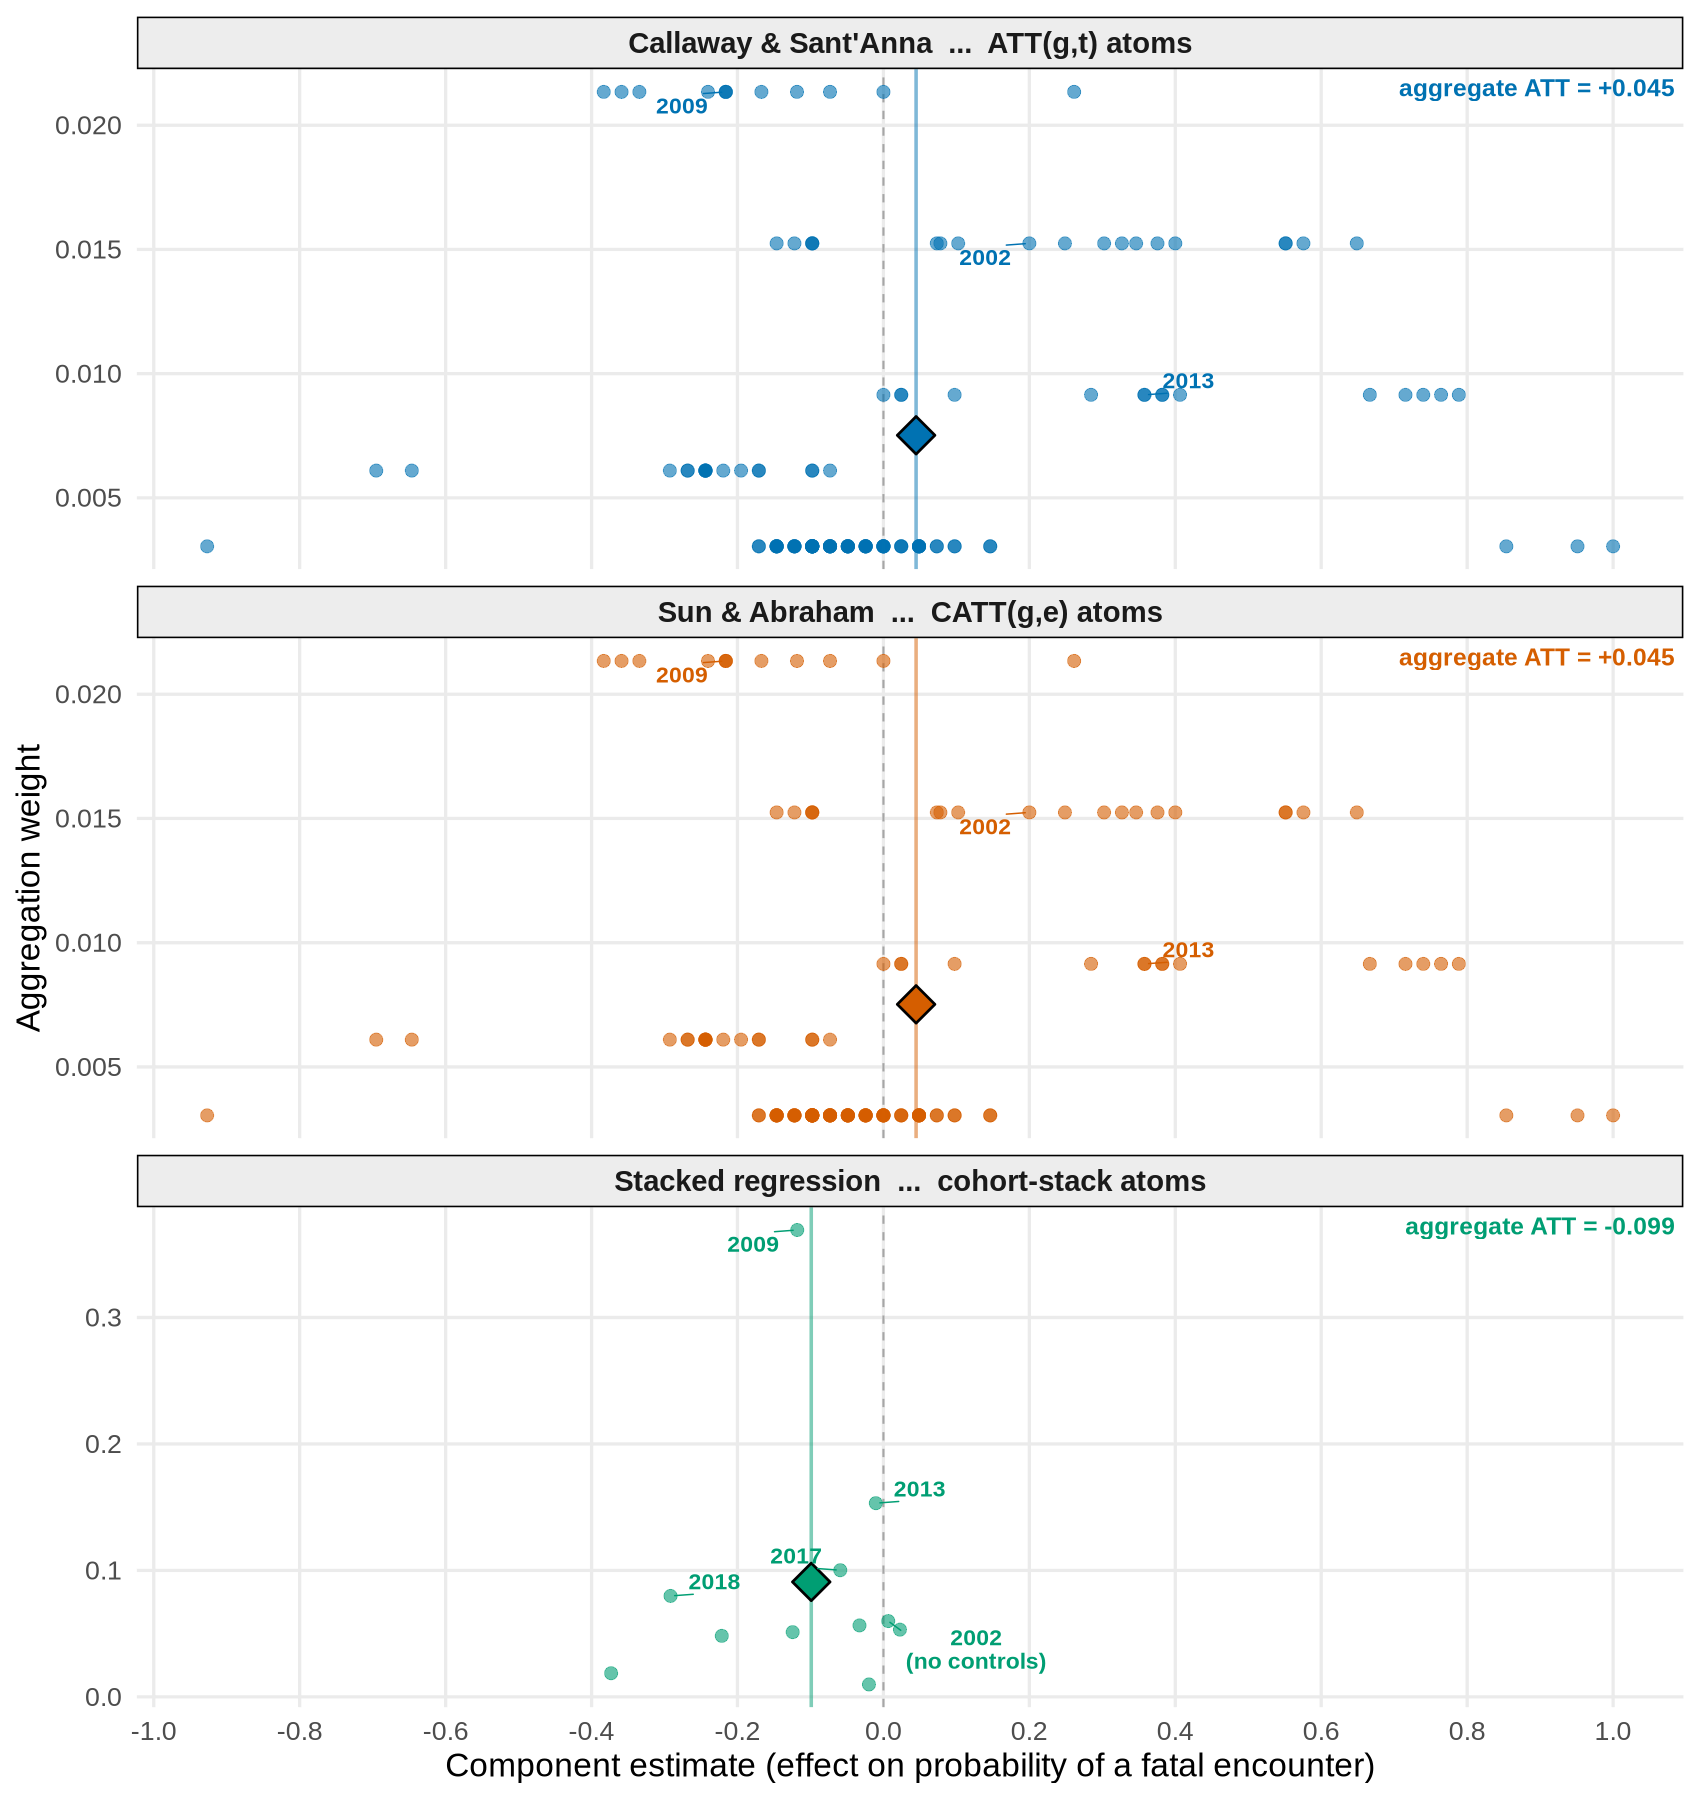
\includegraphics[width=0.6\linewidth]{figures/weight_vs_beta_smallmultiples.png}
        \label{fig:small}
    \end{figure}
\end{frame}

\begin{frame}{What assumptions do they need for their result to hold?}

\begin{table}[]
\centering
\resizebox{\textwidth}{!}{%
\begin{tabular}{|c|c|c|c|}
\hline
Model                                                  & Estimate & SE      & Support Their Results        \\ \hline
Their Specification                                    & $−0.09081$ & $0.00433$ & Yes                          \\ \hline
Remove Covariates                                      & $-0.10440$ & $0.03827$ & Yes                          \\ \hline
Fix agency*stack FE                                    &$ -0.09892$ & $0.03944$ & Yes                          \\ \hline
Fix windowing for stacks                               & $-0.06151$ & $0.06924$ & No, Insignificant            \\ \hline
Fix windowing, not-yet-treated controls                & $-0.06163$ & $0.06921$ & No, Insignificant            \\ \hline
Switch to CS, never-treated controls, full aggregation & $0.04477$  & $0.06503$ & No, sign flip, insignificant \\ \hline
\end{tabular}
}
\end{table}
    
\end{frame}


\end{document}


Run TWFE using always treated units as controls, remove all opposite switchers